\textit{A a planar two link manipulator shown has equal link lengths of 20 and is to move from (6, 0.01) to (-4,0.01) in 0.5 seconds. \\ \\
Generate values for $\theta_1$, $\theta_2$, $\dot{\theta_1}$, $\dot{\theta_2}$ at every 0.025 seconds first using JIM then using CIM. In JIM the joints should reach constant speed in 0.05 s. In CIM the end point should reach constant speed in 0.05 s. Deceleration of each of the parameters should also occur in 0.05 s and use a linear change in speed during both acceleration and deceleration
}
\\
First generate the forward kinematic equations for the manipulator.
\begin{eqnarray}
\phi_1&=&\begin{bmatrix}
\cos(\theta_1)&-\sin(\theta_1)&0&0\\ 
\sin(\theta_1)&\cos(\theta_1)&0&0\\ 
0&0&1&0\\ 
0&0&0&1\\ 
\end{bmatrix} \\
T_1&=&\begin{bmatrix}
1.00&0.00&0.00&20.00\\ 
0.00&1.00&0.00&0.00\\ 
0.00&0.00&1.00&0.00\\ 
0.00&0.00&0.00&1.00\\ 
\end{bmatrix} \\
\phi_2&=&\begin{bmatrix}
\cos(\theta_2)&-\sin(\theta_2)&0&0\\ 
\sin(\theta_2)&\cos(\theta_2)&0&0\\ 
0&0&1&0\\ 
0&0&0&1\\ 
\end{bmatrix} \\
T_2&=&\begin{bmatrix}
1.00&0.00&0.00&20.00\\ 
0.00&1.00&0.00&0.00\\ 
0.00&0.00&1.00&0.00\\ 
0.00&0.00&0.00&1.00\\ 
\end{bmatrix} \\
T_w&=&\begin{bmatrix}
\cos(\theta_1 + \theta_2)&-\sin(\theta_1 + \theta_2)&0&20\cdot \cos(\theta_1 + \theta_2) + 20\cdot \cos(\theta_1)\\ 
\sin(\theta_1 + \theta_2)&\cos(\theta_1 + \theta_2)&0&20\cdot \sin(\theta_1 + \theta_2) + 20\cdot \sin(\theta_1)\\ 
0&0&1&0\\ 
0&0&0&1\\ 
\end{bmatrix} 
\end{eqnarray}


Since we only care about the end position and not orientation we only need the equations for x and y coordinates:
\begin{eqnarray}
x&=&\begin{bmatrix}
20\cdot \cos(\theta_1 + \theta_2) + 20\cdot \cos(\theta_1)\\ 
\end{bmatrix} \\
y&=&\begin{bmatrix}
20\cdot \sin(\theta_1 + \theta_2) + 20\cdot \sin(\theta_1)\\ 
\end{bmatrix} 
\end{eqnarray}


The inverse kinematics for $\theta_1$ can be found by using atan2 to find the angle of the point (x, y) from the world coordinates. ($\hat{\theta} $ in the sketch below). Then use the law of cosines to find the interior angle of the triangle. As drawn the interior angle is always additive to $\hat{\theta}$ to get $\theta_1$, but it can also be oriented in the other direction. $\theta_2$ can be found using atan2 from the end of link 1 to the end of link 2 then subtracting off $\theta_1$ since $\theta_2$ is measured from coordinate frame rotating with the first linkage.

\begin{eqnarray}
\theta_1&=&\tan\parens{\frac{y}{x}}^{-1}+\cos\parens{\frac{l_1^2-l_2^2+x^2+y^2}{2l_1\sqrt{x^2+y^2}}}^{-1} \\
\theta_2&=&\tan\parens{\frac{y-l_1\sin{\theta_1}}{x-l_1\cos{\theta_1}}}^{-1}-\theta_1
\end{eqnarray}

Where $l_1=l_2=20$.

\vspace{4in} 

For the the initial and final points the following joint angles were found:
\begin{center}
	\begin{tabular}{|c|c|c|c|}
	\hline
��������X� & Y��� & $\theta_1$�� & $\theta_2$�� \\ \hline
��������6� & 0.01 & 81.4686$^o$� & 197.2539$^o$ \\  \hline
��������-4 & 0.01 & 264.1176$^o$ & 191.4784$^o$ \\ \hline 
	\end{tabular}
\end{center}

For each of the types of motion the velocity profile must ramp up and then down the area under the velocity curve will be the distance traveled by either the $\theta$s for JIM or the tip (x, y) for CIM.

Divide the constant velocity time steps up into areas of size A*, with magnitude $\dot{Q}_{max}$ and duration $\Delta$.

\begin{eqnarray}
0.25A^*+0.75A^*+16A^*+0.75A^*+0.25A^*=Q_{final}-Q_{initial}
\end{eqnarray}

For all variables $A^*=\frac{\Delta Q}{18}$. The $\delta$ of each variable for each step is given by $0.25A^*$ \& $0.75A^*$ during acceleration and reverse during deceleration. At all points in between it is equal to $A^*$.

\vspace{4in}

\begin{center}
\rowcolors{2}{white}{lightgray}
\begin{table}[H]
	\begin{tabular}{|c|c|c|c|c|c|c|c|c|c|c|c|}
	\hline
\textbf{Step} & \textbf{Time} & \textbf{$\Delta\theta_1$} & \textbf{$\theta_1$} & \textbf{$\Delta\theta_2$} & \textbf{$\theta_2$} & \textbf{X} & \textbf{Y} & \textbf{$\dot{\theta}_1$} & \textbf{$\dot{\theta}_2$} & \textbf{$\dot{X}$} & \textbf{$\dot{Y}$} \\ \hline
0 & 0.000 & 0.000 & 81.469 & 0.000 & 197.254 & 6.000 & 0.010 &  &  &  & \\ \hline
1 & 0.025 & 2.537 & 84.005 & -0.080 & 197.174 & 5.947 & 0.534 & 101.472 & -3.209 & -2.660 & 26.176 \\ \hline
2 & 0.050 & 7.610 & 91.616 & -0.241 & 196.933 & 5.848 & 1.048 & 304.415 & -9.626 & -4.928 & 25.715 \\ \hline
3 & 0.075 & 10.147 & 101.763 & -0.321 & 196.612 & 5.468 & 2.005 & 405.887 & -12.834 & -19.006 & 47.852 \\ \hline
4 & 0.100 & 10.147 & 111.910 & -0.321 & 196.291 & 4.937 & 2.863 & 405.887 & -12.834 & -26.578 & 42.910 \\ \hline
5 & 0.125 & 10.147 & 122.057 & -0.321 & 195.970 & 4.276 & 3.599 & 405.887 & -12.834 & -33.026 & 36.820 \\ \hline
6 & 0.150 & 10.147 & 132.204 & -0.321 & 195.650 & 3.512 & 4.196 & 405.887 & -12.834 & -38.185 & 29.818 \\ \hline
7 & 0.175 & 10.147 & 142.352 & -0.321 & 195.329 & 2.674 & 4.639 & 405.887 & -12.834 & -41.937 & 22.164 \\ \hline
8 & 0.200 & 10.147 & 152.499 & -0.321 & 195.008 & 1.789 & 4.922 & 405.887 & -12.834 & -44.218 & 14.130 \\ \hline
9 & 0.225 & 10.147 & 162.646 & -0.321 & 194.687 & 0.889 & 5.041 & 405.887 & -12.834 & -45.010 & 5.988 \\ \hline
10 & 0.250 & 10.147 & 172.793 & -0.321 & 194.366 & 0.002 & 5.002 & 405.887 & -12.834 & -44.348 & -1.992 \\ \hline
11 & 0.275 & 10.147 & 182.940 & -0.321 & 194.045 & -0.844 & 4.810 & 405.887 & -12.834 & -42.313 & -9.560 \\ \hline
12 & 0.300 & 10.147 & 193.087 & -0.321 & 193.724 & -1.625 & 4.481 & 405.887 & -12.834 & -39.027 & -16.484 \\ \hline
13 & 0.325 & 10.147 & 203.235 & -0.321 & 193.404 & -2.318 & 4.029 & 405.887 & -12.834 & -34.652 & -22.567 \\ \hline
14 & 0.350 & 10.147 & 213.382 & -0.321 & 193.083 & -2.905 & 3.476 & 405.887 & -12.834 & -29.376 & -27.645 \\ \hline
15 & 0.375 & 10.147 & 223.529 & -0.321 & 192.762 & -3.374 & 2.845 & 405.887 & -12.834 & -23.415 & -31.595 \\ \hline
16 & 0.400 & 10.147 & 233.676 & -0.321 & 192.441 & -3.713 & 2.158 & 405.887 & -12.834 & -16.995 & -34.337 \\ \hline
17 & 0.425 & 10.147 & 243.823 & -0.321 & 192.120 & -3.920 & 1.441 & 405.887 & -12.834 & -10.351 & -35.835 \\ \hline
18 & 0.450 & 10.147 & 253.970 & -0.321 & 191.799 & -3.995 & 0.719 & 405.887 & -12.834 & -3.715 & -36.098 \\ \hline
19 & 0.475 & 7.610 & 261.581 & -0.241 & 191.559 & -4.013 & 0.363 & 304.415 & -9.626 & -0.915 & -17.788 \\ \hline
20 & 0.500 & 2.537 & 264.118 & -0.080 & 191.478 & -4.000 & 0.010 & 101.472 & -3.209 & 0.654 & -17.670 \\ \hline
	\end{tabular}
\caption{Joint interpolated motion}
\end{table}
\end{center}
\begin{center}
\rowcolors{1}{white}{lightgray}
\begin{table}[H]
	\begin{tabular}{|c|c|c|c|c|c|c|c|c|c|c|c|}
	\hline
\textbf{Step} & \textbf{Time} & \textbf{$\theta_1$} & \textbf{$\theta_2$} & \textbf{$\Delta X$} & \textbf{X} & \textbf{$\Delta Y$} & \textbf{Y} & \textbf{$\dot{\theta}_1$} & \textbf{$\dot{\theta}_2$} & \textbf{$\dot{X}$} & \textbf{$\dot{Y}$} \\ \hline
0.0 & 0.0 & 81.4686 & 197.2539 & 0.0 & 6.0000 & 0.0 & 0.01 &  &  &  & \\ \hline
1.0000 & 0.0250 & 81.8754 & 196.4494 & -0.1389 & 5.8611 & 0.0 & 0.01 & 16.2746 & -32.1783 & -5.5556 & 0.0\\ \hline
2.0000 & 0.0500 & 82.2823 & 195.6458 & -0.4167 & 5.4444 & 0.0 & 0.01 & 16.2772 & -32.1457 & -16.6667 & 0.0\\ \hline
3.0000 & 0.0750 & 83.0968 & 194.0408 & -0.5556 & 4.8889 & 0.0 & 0.01 & 32.5785 & -64.2002 & -22.2222 & 0.0\\ \hline
4.0000 & 0.1000 & 83.9130 & 192.4385 & -0.5556 & 4.3333 & 0.0 & 0.01 & 32.6458 & -64.0896 & -22.2222 & 0.0\\ \hline
5.0000 & 0.1250 & 84.7323 & 190.8387 & -0.5556 & 3.7778 & 0.0 & 0.01 & 32.7738 & -63.9921 & -22.2222 & 0.0\\ \hline
6.0000 & 0.1500 & 85.5573 & 189.2410 & -0.5556 & 3.2222 & 0.0 & 0.01 & 32.9996 & -63.9074 & -22.2222 & 0.0\\ \hline
7.0000 & 0.1750 & 86.3923 & 187.6452 & -0.5556 & 2.6667 & 0.0 & 0.01 & 33.3994 & -63.8353 & -22.2222 & 0.0\\ \hline
8.0000 & 0.2000 & 87.2460 & 186.0508 & -0.5556 & 2.1111 & 0.0 & 0.01 & 34.1495 & -63.7758 & -22.2222 & 0.0\\ \hline
9.0000 & 0.2250 & 88.1395 & 184.4576 & -0.5556 & 1.5556 & 0.0 & 0.01 & 35.7413 & -63.7285 & -22.2222 & 0.0\\ \hline
10.0 & 0.2500 & 89.1403 & 182.8652 & -0.5556 & 1.0000 & 0.0 & 0.01 & 40.0310 & -63.6930 & -22.2222 & 0.0\\ \hline
11.0000 & 0.2750 & 90.6521 & 181.2736 & -0.5556 & 0.4444 & 0.0 & 0.01 & 60.4728 & -63.6657 & -22.2222 & 0.0\\ \hline
12.0000 & 0.3000 & 264.6974 & 180.3196 & -0.5556 & -0.1111 & 0.0 & 0.01 & 6961.8117 & -38.1596 & -22.2222 & 0.0\\ \hline
13.0000 & 0.3250 & 268.1855 & 181.9102 & -0.5556 & -0.6667 & 0.0 & 0.01 & 139.5244 & 63.6226 & -22.2222 & 0.0\\ \hline
14.0000 & 0.3500 & 267.7802 & 183.5021 & -0.5556 & -1.2222 & 0.0 & 0.01 & -16.2142 & 63.6763 & -22.2222 & 0.0\\ \hline
15.0000 & 0.3750 & 267.1304 & 185.0947 & -0.5556 & -1.7778 & 0.0 & 0.01 & -25.9934 & 63.7058 & -22.2222 & 0.0\\ \hline
16.0000 & 0.4000 & 266.4103 & 186.6884 & -0.5556 & -2.3333 & 0.0 & 0.01 & -28.8036 & 63.7460 & -22.2222 & 0.0\\ \hline
17.0000 & 0.4250 & 265.6600 & 188.2833 & -0.5556 & -2.8889 & 0.0 & 0.01 & -30.0102 & 63.7981 & -22.2222 & 0.0\\ \hline
18.0000 & 0.4500 & 264.8937 & 189.8799 & -0.5556 & -3.4444 & 0.0 & 0.01 & -30.6518 & 63.8626 & -22.2222 & 0.0\\ \hline
19.0000 & 0.4750 & 264.5066 & 190.6789 & -0.4167 & -3.8611 & 0.0 & 0.01 & -15.4832 & 31.9594 & -16.6667 & 0.0\\ \hline
20.0 & 0.5000 & 264.1176 & 191.4784 & -0.1389 & -4.0000 & 0.0 & 0.01 & -15.5626 & 31.9803 & -5.5556 & 0.0\\\hline
	\end{tabular}
\caption{Cartesian interpolated motion}
\end{table}
\end{center}

For both of the tables the velocities of the end effector and joint angles are the average velocity during that step. For example for CIM the average x velocity during step 1 is -5.5556/s, since speed is ramping linearly (constant acceleration) the velocity at the beginning of step 1 is 0/s and at the end is -11.1111/s, for step 2 it starts at  -11.1111/s and ends at -22.2222/s, averaging -16.6667/s, and reaching a constant speed by the end of step 2 (0.05s).

\begin{figure}[H]
  \centering
    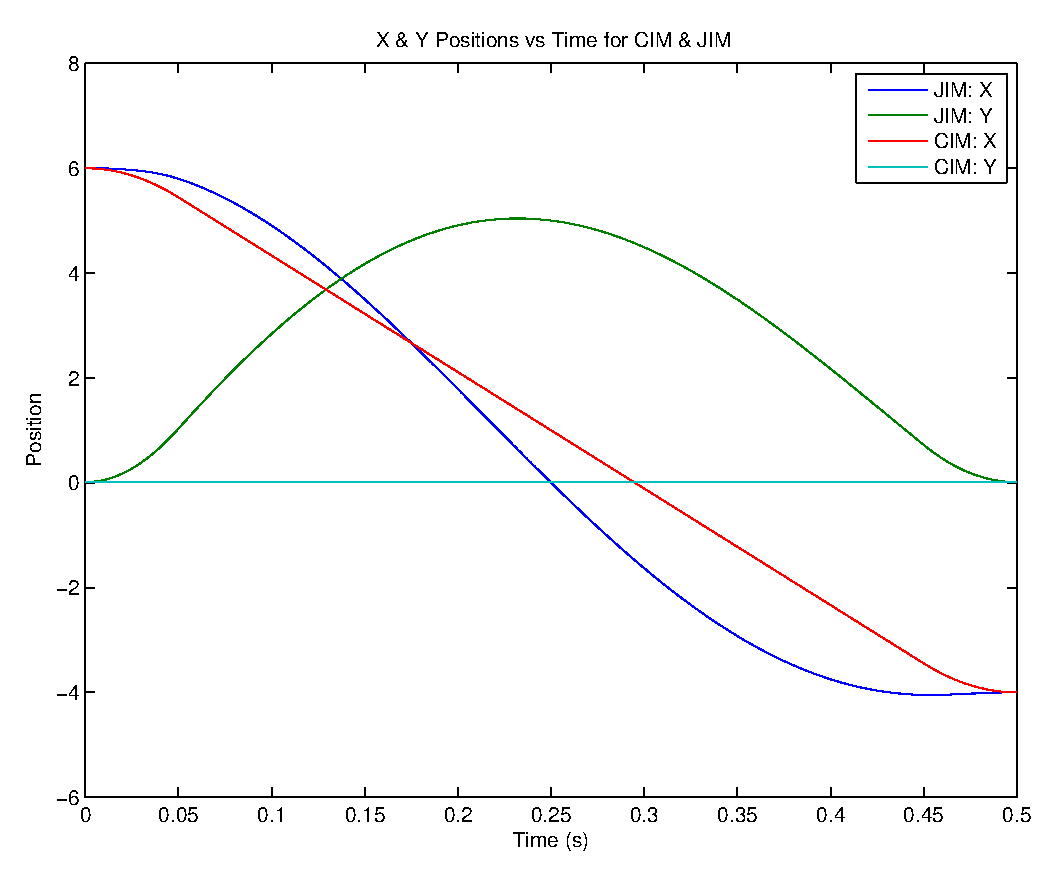
\includegraphics[height=.6\textwidth]{EndPosition}
  \caption{End Position X \& Y coordinates vs time for both types of motion}
  \label{EndPosition}
\end{figure}

\begin{figure}[H]
  \centering
    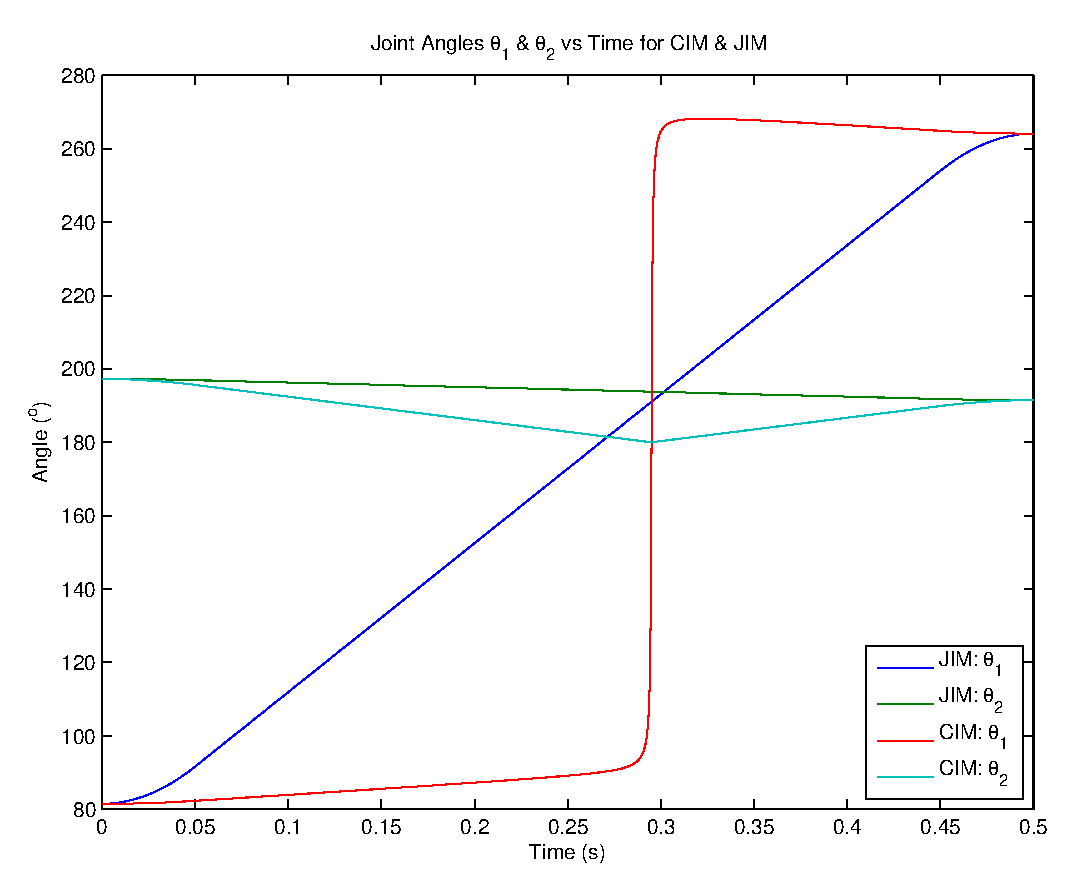
\includegraphics[height=.6\textwidth]{JointAngles}
 \caption{Joint angles $\theta_1$ \& $\theta_2$ vs time for both types of motion}
  \label{JointAngles}
\end{figure}

\begin{figure}[H]
  \centering
    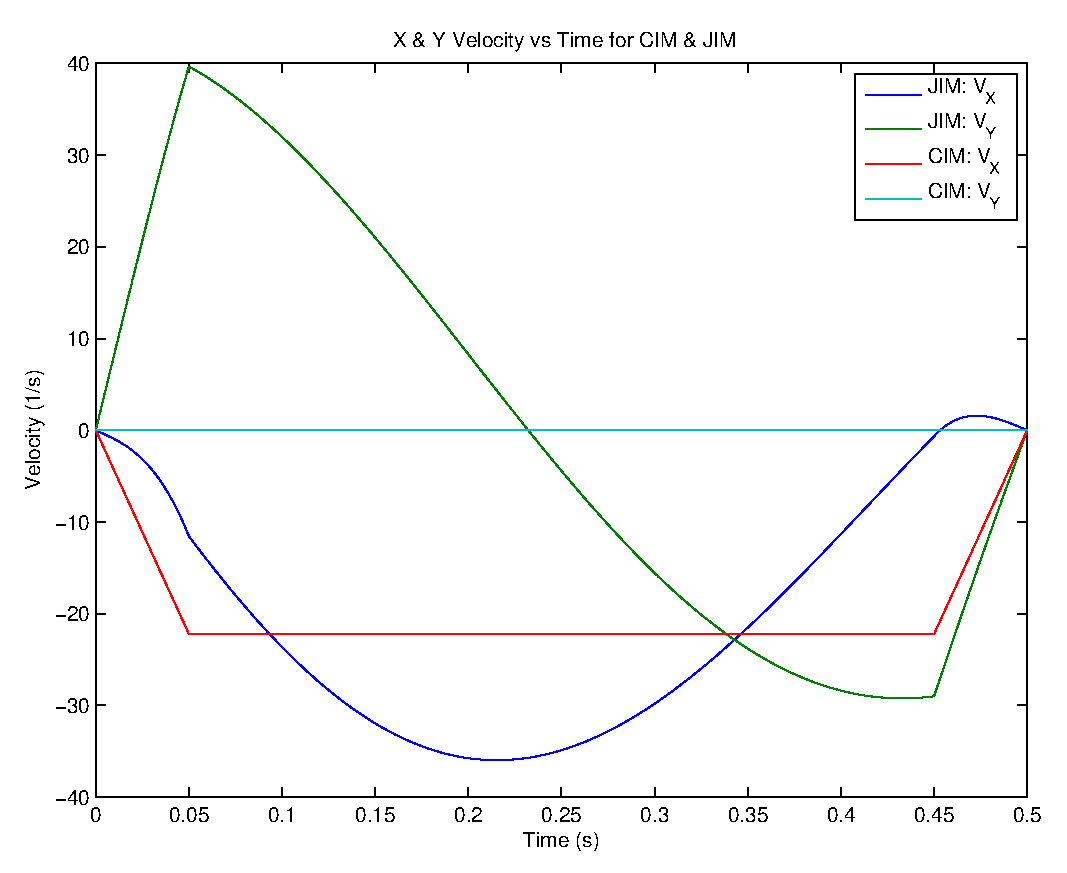
\includegraphics[height=.6\textwidth]{EEVel}
 \caption{Velocity of X \& Y position vs time for both types of motion}
  \label{EEVel}
\end{figure}

\begin{figure}[H]
  \centering
    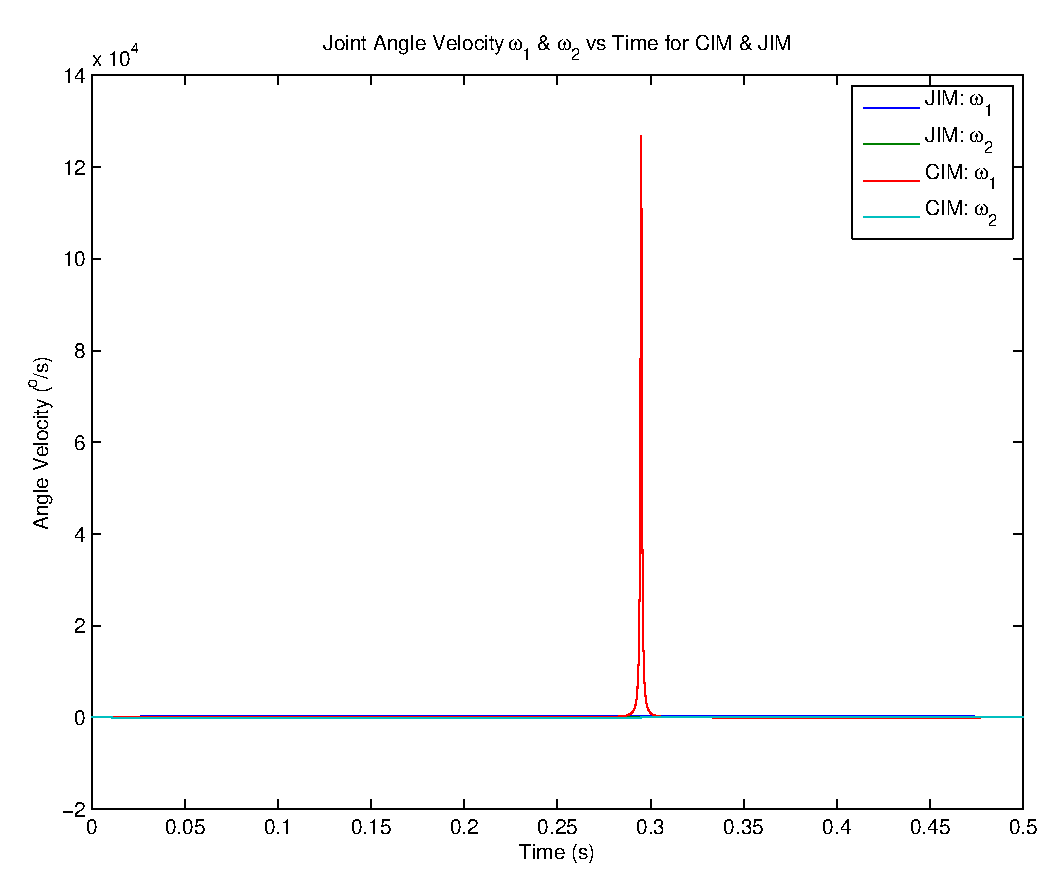
\includegraphics[height=.6\textwidth]{AngleVel}
 \caption{Angular velocity of  $\theta_1$ \& $\theta_2$ position vs time for both types of motion}
  \label{AngleVel}
\end{figure}

\begin{figure}[H]
  \centering
    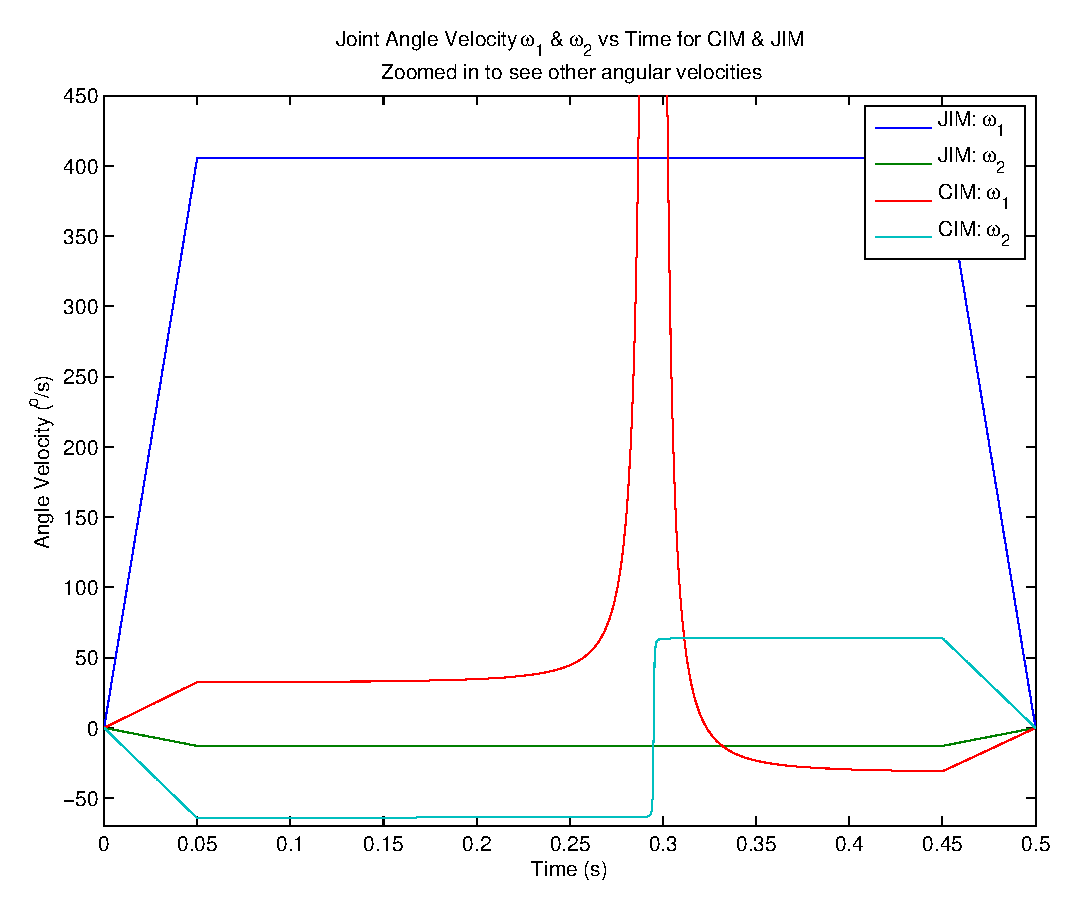
\includegraphics[height=.6\textwidth]{AngleVel2}
 \caption{Angular velocity plot zoomed in to see the detail of the other angular velocities}
  \label{AngleVel2}
\end{figure}

\begin{figure}[H]
  \centering
    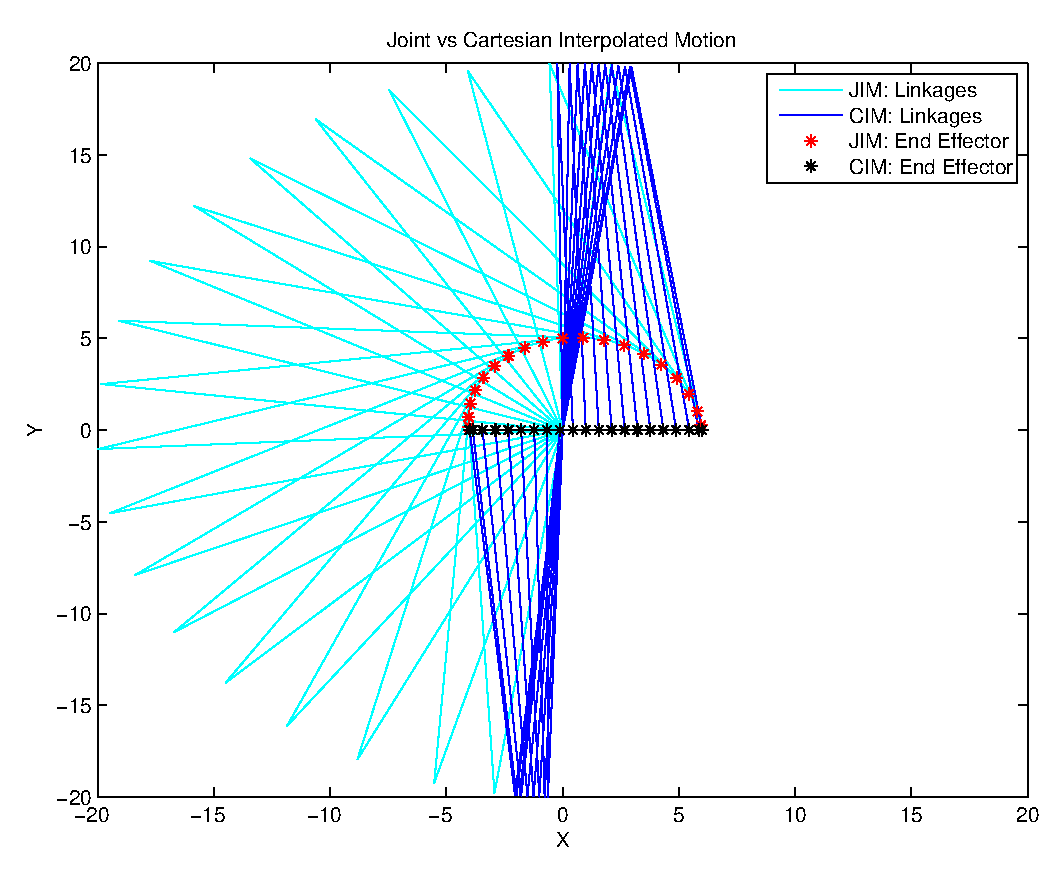
\includegraphics[height=.6\textwidth]{EndEffectorBoth}
 \caption{Manipulator motion in for both types of motion}
  \label{EndEffectorBoth}
\end{figure}

\textit{Comment on the results obtained}

Joint interpolated motion kept the angular velocities of each of the joints reasonable however it didn't follow a straight line path from start to finish. The cartesian interpolated motion followed a straight line from start to finish however since it passed near the singularity the angular velocity of $\theta_1$ spiked as it swung around from quadrant II to III.